\documentclass{article}
\usepackage{fancyhdr}

\setlength{\headheight}{14.5pt}  % Increase headheight to avoid the warning
% Package imports
\usepackage[a4paper, margin=1in]{geometry}
\usepackage{graphicx}
\usepackage{fancyhdr}
\usepackage{titlesec}
\usepackage{titling}
\usepackage{hyperref}
\usepackage{mathastext}
\usepackage{enumitem}
\usepackage{amsmath}
\usepackage{amssymb}
\usepackage{listings}
\usepackage{xcolor}
\usepackage{cancel}
\usepackage{cite}
\newcommand{\bnabla}{\boldsymbol{\nabla}}

% Custom headers and footers
\pagestyle{fancy}
\fancyhf{}
\fancyhead[L]{\leftmark}
\fancyhead[R]{\thepage}

% Define Mathematica language for listings
\lstdefinelanguage{Mathematica}{
  keywords={Plot, Sin, Cos, Table, Module, If, While, For, Do, Switch, Which, Block, Begin, End, Return, Break, Continue},
  sensitive=true,
  morecomment=[l]{(*},
  morecomment=[s]{(*}{*)},
  morestring=[b]"
}

% Customizing the appearance
\lstset{
  language=Mathematica,
  basicstyle=\ttfamily,
  keywordstyle=\color{blue},
  commentstyle=\color{green},
  stringstyle=\color{red},
  numbers=left,
  numberstyle=\tiny\color{gray},
  stepnumber=1,
  numbersep=5pt,
  backgroundcolor=\color{gray!10},
  showspaces=false,
  showstringspaces=false,
  frame=single,
  breaklines=true,
  tabsize=4
}

% Title format customization
\titleformat{\section}
  {\normalfont\Large\bfseries}
  {\thesection}{1em}{}
\titleformat{\subsection}
  {\normalfont\large\bfseries}
  {\thesubsection}{1em}{}

% Hyperlink setup
\hypersetup{
    colorlinks=true,
    linkcolor=blue,
    filecolor=magenta,      
    urlcolor=cyan,
}

% Title and author information
\title{Exploration of Bose-Einstein Condensation in Harmonic Potential Traps}
\author{Youssef Yasser \\ 202101134}
\date{\today}
\numberwithin{equation}{section}
\numberwithin{equation}{subsection}

\begin{document}

% Title page
\begin{titlepage}
    \centering
    \vspace*{2cm}
    
    \Huge
    \textbf{Exploration of Bose-Einstein Condensation in Harmonic Potential Traps}
    
    \vspace{0.5cm}
    \LARGE
    
    
    \vspace{1.5cm}
    
    \textbf{Youssef Yasser 202101134}\\
    \textbf{Hazem Mohamed 202200777}
    
    %\vfill
    
    
    
    \vspace{1.5cm}
    
\includegraphics[width=0.7\textwidth]{zewailcity logo.jpg}

    \Large
    PEU 311 - Statistical Physics\\
    Dr. Amr Sweyllam
\end{titlepage}

\newpage
\tableofcontents
\newpage
\begin{abstract}
    In this project, we explore the properties of a bosonic gas subjected to harmonic potential traps, both isotropic and anisotropic, near the temperature of Bose-Einstein condensation.
     We derive expressions for the density of states for both isotropic and anisotropic cases, the condensation temperature and key thermodynamic quantities, focusing on the behavior of the ground-state particle population and the other thermodynamic quantities as the system approaches condensation.
     The condensation fraction and specific heat are calculated to reveal insights into the effects of trap anisotropy on the condensation process. 
\end{abstract}

\section{Introduction}

Bose-Einstein condensation is a physical phenomena that occurs when the system is cooled to temperature near 0k and the particles of the system start to occupy the ground state.
 When a Bose-Einstein condensate (BEC) forms, a macroscopic number of particles occupy the same quantum ground state.
  In this state, the wavefunctions of the individual particles overlap significantly and become coherent.
   The system can then be described by a macroscopic wavefunction, which represents the collective quantum state of the condensate.
    This macroscopic wavefunction is not simply the wavefunction of a single particle but rather a coherent superposition that describes the entire condensate.\\

Albert Einstein predicted this phenomena in 1924-1925 based on the work of Satyendra Nath Bose on quantum statistics.
 In 1995, the Bose–Einstein condensate was created by Eric Cornell and Carl Wieman of the University of Colorado Boulder using rubidium atoms; later that year, Wolfgang Ketterle of MIT produced a BEC using sodium atoms.
  In 2001 Cornell, Wieman, and Ketterle shared the Nobel Prize in Physics "for the achievement of Bose–Einstein condensation in dilute gases of alkali atoms, and for early fundamental studies of the properties of the condensates".\\

  This study focuses on Bose-Einstein condensation (BEC) in three-dimensional anisotropic harmonic traps. The primary goals are to derive the condensation temperature, investigate the behavior of the ground-state particle population near this temperature, and calculate critical thermodynamic quantities such as the condensate fraction and specific heat. Anisotropic traps introduce asymmetry into the confining potential, leading to unique modifications in the condensation process and the thermodynamic properties of the system.\\

  Understanding BEC in anisotropic traps is crucial for several reasons. Unlike isotropic traps, which assume identical confinement along all axes, anisotropic traps reflect the more realistic scenarios encountered in laboratory setups, where the trapping frequencies differ. This asymmetry significantly influences the energy spectrum, altering the critical temperature and the distribution of particles between the ground and excited states. Such studies provide essential insights into the dynamics of confined bosonic gases, aiding in the refinement of theoretical models and experimental designs.\\
  
  The implications of this research extend beyond atomic physics. By studying bosons in harmonic potentials, we can gain a deeper understanding of collective quantum phenomena, which are vital for developing applications in quantum technologies, such as atom interferometry, quantum simulations, and high-precision measurements. Furthermore, the behavior of BEC in anisotropic traps has parallels with phenomena in quantum field theories, making these systems a valuable platform for modeling early-universe physics, including symmetry breaking and phase transitions.\\
  
  This project employs a combination of analytical techniques and approximations to derive expressions for the condensation temperature and other thermodynamic quantities. The study explores how varying the trap anisotropy affects the condensate fraction and specific heat, particularly near the condensation temperature. Additionally, by examining the interplay between trap geometry and quantum degeneracy, this work aims to identify conditions that optimize condensate stability and coherence, contributing to future experimental advancements.\\
  

\section{Calculating Density of States}
  In this section we are computing the density of states that is essential to us in our analysis and to derive the key thermodynamic quantities that we are interested in. First of all let us define the potential of the system and its corresponding energies. 
  The system is subjected to the potential of the form:
  \begin{equation}
    V_{ext}(\mathbf{r})=\frac{m}{2}(\omega_{\mathit{x}}x^2+\omega_{\mathit{y}}y^2+\omega_{\mathit{z}}z^2)
  \end{equation}
  In isotropic case, $\omega_{\mathit{x}} = \omega_{\mathit{y}} = \omega_{\mathit{z}}$ while in anisotropic case $\omega_{\mathit{x}} \neq \omega_{\mathit{y}} \neq \omega_{\mathit{z}}$. The corresponding eigenenergies of the Hamiltonian with this potential are 
  \begin{equation}
    \varepsilon_{\mathit{n}_{\mathit{x}},\mathit{n}_{\mathit{y}},\mathit{n}_{\mathit{z}}} = \hbar\left(\omega_{\mathit{x}}\left(\mathit{n}_{\mathit{x}}+\frac{1}{2}\right)+\omega_{\mathit{y}}\left(\mathit{n}_{\mathit{y}}+\frac{1}{2}\right)+\omega_{\mathit{z}}\left(\mathit{n}_{\mathit{z}}+\frac{1}{2}\right)\right)
  \end{equation}
Using these eigenenergies we can compute the density of states for both isotropic and anisotropic cases.\\

Firstly, before computing the DOSs, we must start by a crucial argument on the ground state contribution of the eigenvalues of the Hamiltonian and how can we ignore this part. This is imortant because this will simplufy the analysis effectively.
\subsection{Discusion on Neglecting The Ground State Contribution Term}
\subsubsection{Energy Spectrum in Harmonic Traps}
For a boson gas confined in an anisotropic harmonic trap, the single-particle energy levels are given by:
\[
    \varepsilon_{\mathit{n}_{\mathit{x}},\mathit{n}_{\mathit{y}},\mathit{n}_{\mathit{z}}} = \hbar\left(\omega_{\mathit{x}}\left(\mathit{n}_{\mathit{x}}+\frac{1}{2}\right)+\omega_{\mathit{y}}\left(\mathit{n}_{\mathit{y}}+\frac{1}{2}\right)+\omega_{\mathit{z}}\left(\mathit{n}_{\mathit{z}}+\frac{1}{2}\right)\right)
\]
where \( \mathit{n}_{\mathit{x}},\mathit{n}_{\mathit{y}},\mathit{n}_{\mathit{z}} \) are non-negative integers (quantum numbers of the system). The term \( \frac{1}{2} \hbar (\omega_{\mathit{x}} + \omega_{\mathit{y}} + \omega_{\mathit{z}}) \) represents the ground state energy of the harmonic trap.

\subsubsection{Recalling what Density of States (DOS) is}
The density of states (DOS), \( g(E) \), describes the number of states available per unit energy interval. It is derived by counting the total number of states below a given energy \( E \). For the anisotropic trap:
\[
g(E) = \frac{d}{dE} \int_{\text{all states}} \delta(E - E_{\mathit{n}_{\mathit{x}},\mathit{n}_{\mathit{y}},\mathit{n}_{\mathit{z}}}) \, dE.
\]
This calculation depends on the spacing between energy levels and their degeneracy, not the absolute values of energy.

\subsubsection{Shifting the Zero Point of Energy}
The ground state energy \( \frac{1}{2} \hbar (\omega_{\mathit{x}} + \omega_{\mathit{y}} + \omega_{\mathit{z}}) \) adds a constant offset to all energy levels. Mathematically:
\[
E_{\mathit{n}_{\mathit{x}},\mathit{n}_{\mathit{y}},\mathit{n}_{\mathit{z}}} = \tilde{E}_{\mathit{n}_{\mathit{x}},\mathit{n}_{\mathit{y}},\mathit{n}_{\mathit{z}}} + E_{\text{GS}},
\]
where \( \tilde{E}_{\mathit{n}_{\mathit{x}},\mathit{n}_{\mathit{y}},\mathit{n}_{\mathit{z}}} = \hbar (\mathit{n}_{\mathit{x}} \omega_{\mathit{x}} + \mathit{n}_{\mathit{y}} \omega_{\mathit{y}} + \mathit{n}_{\mathit{z}} \omega_{\mathit{z}}) \) is the shifted energy spectrum, and \( E_{\text{GS}} = \frac{1}{2} \hbar (\omega_{\mathit{x}} + \omega_{\mathit{y}} + \omega_{\mathit{z}}) \) is the ground state energy.\\

The DOS is derived from the distribution of states over energy differences. Since the DOS depends on the derivative of the cumulative number of states:
\[
g(E) = \frac{dN(E)}{dE},
\]
shifting the spectrum by \( E_{\text{GS}} \) affects neither the distribution of states \( N(E) \) nor its derivative. Only the absolute reference point of the energy changes, not the relative distribution of states.

\subsubsection{Impact on Thermodynamic Quantities}
Thermodynamic quantities like the partition function \( Z \) depend on the energy spectrum. When \( E_{\text{GS}} \) is included, it adds a constant multiplicative factor:
\[
Z = e^{-\beta E_{\text{GS}}} \tilde{Z},
\]
where \( \tilde{Z} \) is the partition function calculated using the shifted spectrum \( \tilde{E}_{\mathit{n}_{\mathit{x}},\mathit{n}_{\mathit{y}},\mathit{n}_{\mathit{z}}} \). However, this constant factor cancels out in most thermodynamic derivatives, such as the free energy, entropy, and specific heat. Hence, ignoring \( E_{\text{GS}} \) simplifies calculations without altering the physical predictions.

\subsubsection{Why the DOS Remains Unchanged}
The DOS is fundamentally a measure of the energy-level density in phase space. It is invariant under a constant shift of all energy levels because the shift does not change the spacing or degeneracy of the levels.\\

Mathematically, if \( g(E) \) is computed for \( \tilde{E} = E - E_{\text{GS}} \), the form of \( g(\tilde{E}) \) is identical to \( g(E) \) because:
\[
g(E) = \frac{dN}{dE} \quad \text{and} \quad g(\tilde{E}) = \frac{dN}{d\tilde{E}}.
\]
Since \( dE = d\tilde{E} \), the functional relationship remains unchanged.
Thus we can now say that the energy dicrete spectrum is given by
\begin{equation}
    \varepsilon_{\mathit{n}_{\mathit{x}},\mathit{n}_{\mathit{y}},\mathit{n}_{\mathit{z}}}  = \hbar(\omega_{\mathit{x}} \mathit{n}_{\mathit{x}} + \omega_{\mathit{y}} \mathit{n}_{\mathit{y}} + \omega_{\mathit{z}} \mathit{n}_{\mathit{z}})
\end{equation}
And now we are fully ready to compute the DOS, both for Isotroic and anisotropic potentials.

\subsection{Isotropic Potential}
In this case we are assuming $\omega_{\mathit{x}} = \omega_{\mathit{y}} = \omega_{\mathit{z}} = \omega$. Hence the eigenenergies are
\begin{equation}
    \varepsilon_{\mathit{n}_{\mathit{x}},\mathit{n}_{\mathit{y}},\mathit{n}_{\mathit{z}}} = \hbar\omega\left(\mathit{n}_{\mathit{x}}+\mathit{n}_{\mathit{y}}+\mathit{n}_{\mathit{z}}+\frac{3}{2}\right)
\end{equation}
Now define $ \mathit{n} = \mathit{n}_{\mathit{x}}+\mathit{n}_{\mathit{y}}+\mathit{n}_{\mathit{z}}$. Thus,
\begin{equation}
    \varepsilon_{\mathit{n}_{\mathit{x}},\mathit{n}_{\mathit{y}},\mathit{n}_{\mathit{z}}} = \hbar\omega\left(\mathit{n}+\frac{3}{2}\right) \Longrightarrow \mathit{n} = \frac{\varepsilon}{\hbar\omega}-\frac{3}{2}
\end{equation}
We note that the energy is composed of two parts, one for the excitation states ($\mathit{n} > 0 \rightarrow \varepsilon = \mathit{n}\hbar\omega$) and one for the ground state $\left(\mathit{n} = 0 \ \rightarrow \varepsilon = \frac{3}{2}\hbar\omega\right)$. For sake of simplicity, we can ignore the ground state contribution term, as we discused previously, but we will first explore the analysis considering the gorund state correction.
the degeneracy of states is given by the number of ways of distributing ($\mathit{n}_{\mathit{x}}, \mathit{n}_{\mathit{y}}, \mathit{n}_{\mathit{z}}$) so their sum is $\mathit{n}$. This degeneracy function is:
\begin{equation}
    D(\mathit{n}) = \frac{(\mathit{n}+2)!}{\mathit{n}!2!}
\end{equation}
for the semiclassical limit where $\mathit{n}>>1$
\begin{equation}
    D(\mathit{n}) \thickapprox  \frac{\mathit{n}^2}{2}
\end{equation}
To get the total number of states up to energy E, we must count all the possible combination of ($\mathit{n}_{\mathit{x}}, \mathit{n}_{\mathit{y}}, \mathit{n}_{\mathit{z}}$) in every energy level. This is done by summing eqn(2.1.3) but we assume semiclassical limit so insterad of discrete sum we are perfoming an integral on eqn(2.1.4) to get to total number of states $G(n)$. The lower limit of integration is clearly 0 and the upper limit, by virtue of eqn(2.1.2), is $\mathit{n} = \frac{E}{\hbar\omega}-\frac{3}{2} $. Thus, The total number of states is:
\begin{equation}
    G(\mathit{E}) = \int_{0}^{(\frac{E}{\hbar\omega}-\frac{3}{2})} \frac{\mathit{n}^2}{2} \,d\mathit{n} = \left(\frac{\mathit{n}^3}{6}\right)\bigg|_{0}^{(\frac{E}{\hbar\omega}-\frac{3}{2})} = \frac{1}{6}\left(\frac{E}{\hbar\omega}-\frac{3}{2}\right)^3
\end{equation}
Therefore, the density of states (DOS) is 
\begin{equation}
    g(\mathit{n}) = \frac{d}{d E}G(\mathit{E}) = \frac{3}{6}\left(\frac{E}{\hbar\omega}-\frac{3}{2}\right)^2\left(\frac{1}{\hbar \omega}\right)
\end{equation}
Note that if we were to ignore the ground state correction we would have
\begin{equation}
    g(\mathit{n}) = \frac{E^2}{2(\hbar\omega)^3}
\end{equation}

\subsection{Anisotropic Potential}
Here we are assuming $\omega_{\mathit{x}} \neq \omega_{\mathit{y}} \neq \omega_{\mathit{z}}$ and we will drop the ground state contribution term for simplicity. We want to count all the states up tp energy E. For a fixed total energy \(E\), the quantum states correspond to integer triplets \((\mathit{n}_{\mathit{x}},\mathit{n}_{\mathit{y}},\mathit{n}_{\mathit{z}})\) satisfying:

\[
\omega_{\mathit{x}} \mathit{n}_{\mathit{x}} + \omega_{\mathit{y}} \mathit{n}_{\mathit{y}} + \omega_{\mathit{z}} \mathit{n}_{\mathit{z}} \leq \frac{E}{\hbar}.
\]


For large \(E\), the quantum states become dense, and we can approximate the sum over discrete states by the volume of a continuous region in \((\mathit{n}_{\mathit{x}}, \mathit{n}_{\mathit{y}}, \mathit{n}_{\mathit{z}})\)-space. The inequality:
\[
\omega_{\mathit{x}} \mathit{n}_{\mathit{x}} + \omega_{\mathit{y}} \mathit{n}_{\mathit{y}} + \omega_{\mathit{z}} \mathit{n}_{\mathit{z}} \leq \frac{E}{\hbar}.
\]
% After rearranging this inequality, we get,
% \begin{equation}
%     \omega_{\mathit{x}}\mathit{n}_{\mathit{x}}+\omega_{\mathit{y}}\mathit{n}_{\mathit{y}}+\omega_{\mathit{z}}\mathit{n}_{\mathit{z}} \leq \frac{E}{\hbar} - \frac{1}{2}(\omega_{\mathit{x}}+\omega_{\mathit{y}}+\omega_{\mathit{z}})
% \end{equation}
defines a tetrahedron in the first octant, where \(\mathit{n}_{\mathit{x}}, \mathit{n}_{\mathit{y}}, \mathit{n}_{\mathit{z}} \geq 0\).
The tetrahedron is bounded by the planes:
\[
\mathit{n}_{\mathit{x}} = 0, \quad \mathit{n}_{\mathit{y}} = 0, \quad \mathit{n}_{\mathit{z}} = 0, \quad \text{and} \quad \omega_{\mathit{x}} \mathit{n}_{\mathit{x}} + \omega_{\mathit{y}} \mathit{n}_{\mathit{y}} + \omega_{\mathit{z}} \mathit{n}_{\mathit{z}} = \frac{E}{\hbar}.
\]
The vertices of the tetrahedron are:
\[
(0, 0, 0), \quad \left( \frac{E}{\hbar \omega_{\mathit{x}}}, 0, 0 \right), \quad \left( 0, \frac{E}{\hbar \omega_{\mathit{y}}}, 0 \right), \quad \left( 0, 0, \frac{E }{\hbar \omega_{\mathit{z}}} \right).
\]
The volume of a tetrahedron is given by:
\[
\text{Volume} = \frac{1}{6} \cdot \text{Base Area} \cdot \text{Height}.
\]
The base is the triangle formed by the points:
\[
\left( \frac{E }{\hbar \omega_{\mathit{x}}}, 0, 0 \right), \quad \left( 0, \frac{E }{\hbar \omega_{\mathit{y}}}, 0 \right), \quad \text{and} \quad (0, 0, 0).
\]
The area of this triangle is:
\[
\text{Base Area} = \frac{1}{2} \cdot \frac{E }{\hbar \omega_{\mathit{x}}} \cdot \frac{E}{\hbar \omega_{\mathit{y}}} = \frac{E^2}{2\hbar^2\omega_{\mathit{x}}\omega_{\mathit{y}}}.
\]
The height of the tetrahedron is the perpendicular distance from the base which is \[h = \left(\frac{E}{\hbar\omega_{\mathit{z}}}\right)\]\\
Therefore, the volume of the tetrahedron, which is the total number of states up to energy E, is
\begin{equation}
    G(E) = \frac{E^3}{6\hbar^3\omega_{\mathit{x}}\omega_{\mathit{y}}\omega_{\mathit{z}}}
\end{equation} 
Now let us define the geometric mean of the frequencies 
\begin{equation}
    \Omega = \sqrt[3]{\omega_{\mathit{x}}\omega_{\mathit{y}}\omega_{\mathit{z}}}
\end{equation}
And the DOS is the derivative of the total number of states with respect to E, which is
\begin{equation}
    g(\mathit{n}) = \frac{E^2}{2(\hbar\Omega)^3}
\end{equation} 
Note that eqn(2.3.3) is the same as eqn(2.2.7) if we consider the isotropic case.


\section{Calculating the Condensation Tempreature}
To determine the condensation temperature \( T_c \) for a Bose-Einstein condensate confined in an anisotropic harmonic potential, we begin by analyzing the distribution of particles among the quantum states. At temperatures above \( T_c \), all particles occupy excited states, while below \( T_c \), a macroscopic number of particles condense into the ground state. The number of excited particles can be calculated by integrating the Bose-Einstein distribution over the density of states specific to the anisotropic trap. The condensation temperature is then obtained by equating the total number of particles \( N \) to the number of excited particles, as the ground-state population becomes negligible near \( T_c \). This calculation provides the critical temperature marking the onset of Bose-Einstein condensation.\\

The excited-state population is given by the integral of Bose-Einstein distribution function with the DOS:
\begin{equation}
    N_{ex} = \int_{E_G}^{\infty}   \frac{g(\varepsilon)}{e^{\beta (\varepsilon - \mu)} - 1} \,d\varepsilon = \frac{1}{2(\hbar\Omega)^3}\int_{E_G}^{\infty}   \frac{\varepsilon^2}{e^{\beta (\varepsilon - \mu)} - 1} \,d\varepsilon
\end{equation}
where \( E_G \) is the ground state energy, \( \mu \) is the chemical potential, and \( \beta = \frac{1}{k_B T} \) is the inverse temperature.
We now introduce a the fugacity. The fugacity \( Z = e^{\beta \mu} \), where \( \beta = \frac{1}{k_B T} \) and \( \mu \) is the chemical potential, is a dimensionless parameter that provides insight into the thermodynamic properties of a system of particles. It quantifies the deviation of the system from ideal behavior and is particularly significant in Bose-Einstein condensation. For a system of non-interacting bosons, the fugacity is directly related to the particle distribution across quantum states.\\
When \( Z < 1 \), the chemical potential \( \mu \) is negative, and the system is dominated by thermal excitations, with particles spread across many states. As \( Z \to 1^- \), corresponding to \( \mu \to 0^- \), the system approaches the critical conditions for Bose-Einstein condensation, where a macroscopic number of particles begin to occupy the ground state. The fugacity, therefore, serves as a critical parameter in characterizing the transition and the population of quantum states within the system.\\

Now we make the substitution \( x = \beta\varepsilon\) to simplify the integral:
$$N_{ex} = \frac{Z}{2(\beta\hbar\Omega)^3} \int_{x_G}^{\infty} \frac{x^2}{e^x - 1} \,dx
$$

but since we are assuming $E_G = 0$ and hence $x_G = 0$. The integral can be computed using the following Mathematica code:
\begin{lstlisting}[language=Mathematica]
    Integrate[x^2/(Exp[x] - 1), {x, 0, Infinity}]
\end{lstlisting}
and the result is $2\zeta(3)$. Therefore, the total number of excited particles is:
\begin{equation}
    N_{ex} = \frac{Z}{2(\beta\hbar\Omega)^3} 2\zeta(3) = \frac{Z\zeta(3)}{(\beta\hbar\Omega)^3}
\end{equation}

and since near the condensation temperature, $\mu = 0$ and $Z = 1$, the total number of particles is:
\begin{equation}
    N = N_{ex} + N_0 = \zeta(3) \left(\frac{k_BT}{\hbar\Omega}\right)^3  + N_0 
\end{equation}

where $N_0$ is the number of particles in the ground state. The condensation temperature is obtained by setting $N_0 = 0$ and solving for $T$:
\begin{equation}
    T_c = \frac{\hbar\Omega}{k_B}\left(\frac{N}{\zeta(3)}\right)^{1/3}
\end{equation}

\section{Calculating the Condensation Fraction}
The condensation fraction \( N_0/N \) quantifies the proportion of particles that occupy the ground state relative to the total number of particles in the system. This fraction is a key indicator of the onset of Bose-Einstein condensation, as it reveals the transition from a thermal distribution to a macroscopic occupation of the ground state. The condensation fraction is calculated by dividing the number of particles in the ground state by the total number of particles. Near the condensation temperature, the condensation fraction approaches unity, indicating the dominance of the ground state population.\\

To investigate the behavior of the condensation fraction, we refer to eqn(3.0.3) and write an expression for $\frac{N_0}{N}$ as a function of $\frac{T}{T_c}$:
\begin{equation}
    \frac{N_0}{N} = 1 - \left(\frac{T}{T_c}\right)^3
\end{equation}
\begin{center}
    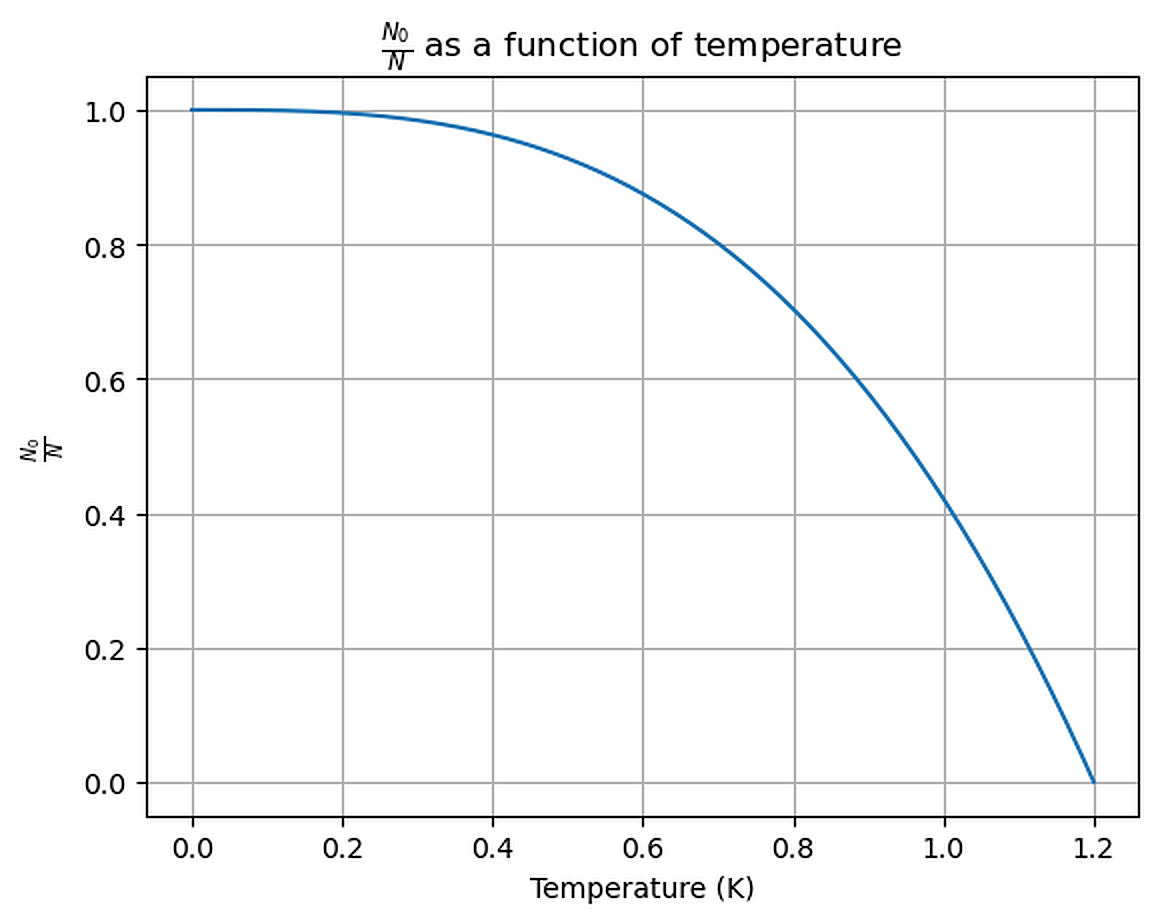
\includegraphics[width=0.7\textwidth]{N_0N_graph_high_quality.png}  
\end{center}
The graph above shows the behavior of the condensation fraction as a function of the reduced temperature \( T/T_c \) assuming $N = 10^{23}$ and $T_c = 1.2k$. Near the condensation temperature, the condensation fraction rapidly increases, approaching unity as \( T \to 0 \). 

\section{The Specific Heat}
The specific heat \( C_V \) characterizes the heat capacity of a system and provides insights into the energy required to raise the temperature by a small amount. In the context of Bose-Einstein condensation, the specific heat near the condensation temperature exhibits unique behavior, reflecting the transition from a thermal distribution to a condensed state. The specific heat is calculated by differentiating the total energy with respect to temperature, yielding the energy required to increase the temperature by a small amount.\\
\subsection{Calculating the Internal Energy}

$$C_V = \frac{dU}{dT}$$
where \( U \) is the internal energy of the system. The internal energy is given by the sum of the energy of the excited particles and the ground-state energy:
\begin{equation}
    U = \int_{E_G}^{\infty} \varepsilon g(\varepsilon) \frac{1}{e^{\beta(\varepsilon - \mu)} - 1} \,d\varepsilon + N_0 E_0
\end{equation}
And since we assume $E_G = 0$, the internal energy is:
\begin{equation}
    U = \int_{0}^{\infty} \varepsilon g(\varepsilon) \frac{1}{e^{\beta(\varepsilon - \mu)} - 1} \,d\varepsilon = \frac{1}{2Z(\hbar\Omega)^3} \int_{0}^{\infty} \frac{\varepsilon^3}{e^{\beta\varepsilon} - 1} \,d\varepsilon
\end{equation}
Now we make the substitution \( x = \beta\varepsilon\) to simplify the integral:
$$U = \frac{1}{2Z(\beta\hbar\Omega)^3} \int_{0}^{\infty} \frac{x^3}{e^x - 1} \,dx = \frac{1}{2Z\beta^4(\hbar\Omega)^3} 3!\zeta(4) = \frac{3!\zeta(4)}{2Z\beta^4(\hbar\Omega)^3} =   \left(\frac{3\zeta(4)}{\hbar^3\Omega^3}\right) \left(\frac{k_b^4T^4}{Z}\right) 
$$
Therefore, the internal energy is:
\begin{equation}
    U = \frac{3\zeta(4)}{\hbar^3\Omega^3} \left(\frac{k_b^4T^4}{Z}\right)
\end{equation}
where \( \zeta(4) \) is the Riemann zeta function evaluated at 4, and $Z = e^{\mu/k_bT}$ is the fugacity. Also near the condensation temperature, $\mu = 0$ and $Z = 1$, the internal energy is:   
\begin{equation}
    U = \frac{3\zeta(4)}{\hbar^3\Omega^3} \left(k_b^4T^4\right) 
\end{equation}
and If T is far from the condensation temperature, the internal energy is:
\begin{equation}
    U = \frac{3\zeta(4)}{\hbar^3\Omega^3} k_b^4T^4\exp\left(\frac{-\mu}{k_bT}\right)
\end{equation}


\subsection{Calculating the Specific Heat}
The specific heat near the condensation temperature is obtained by differentiating eqn(5.1.4) with respect to temperature:
\begin{equation}
    C_V = \frac{dU}{dT} = \frac{12\zeta(4)}{\hbar^3\Omega^3}k_b^4T^3
\end{equation}
Expressing this in terms of the reduced temperature \( T/T_c \) we get:
\begin{equation}
    C_V = \frac{12\zeta(4) N k_b}{\zeta(3)} \left(\frac{T}{T_c}\right)^3
\end{equation}
Introducing the dimensionless parameter \( x = \frac{T}{T_c} \), the specific heat is expressed as:
\begin{equation}
    C_V = \frac{12\zeta(4) N k_b}{\zeta(3)} \left(x\right)^3
\end{equation}

and far from the condensation temperature, the specific heat is obtained by differentiating eqn(5.1.5) with respect to temperature:
\begin{equation}
    C_V = \left(\frac{3\zeta(4)}{\hbar^3\Omega^3}\right) \frac{d}{dT}\left(k_b^4T^4\exp\left(\frac{-\mu}{k_bT}\right)\right) 
\end{equation}
Therefore, the specific heat is:
\begin{equation}
    C_V = \left(\frac{3\zeta(4)}{\hbar^3\Omega^3}\right) \left(4k_b^4T^3\exp\left(\frac{-\mu}{k_bT}\right) - k_b^4T^4\exp\left(\frac{-\mu}{k_bT}\right)\left(\frac{-\mu}{k_bT^2}\right)\right)
\end{equation}
After simplifying the above equation, we get:
\begin{equation}
    C_V = \left(\frac{3\zeta(4)}{\hbar^3 \Omega^3}\right) k_b^4  \left( 4T^3 + \frac{\mu}{k_b} T^2 \right) \exp\left(-\frac{\mu}{k_B T}\right)
\end{equation}

expressing this in terms of the reduced temperature \( T/T_c \) we get:
\begin{equation}
    C_V = \frac{3\zeta(4) N k_b}{\zeta(3)}  \left( 4\left(\frac{T}{T_c}\right)^3 + \frac{\mu}{k_b T_c} \left(\frac{T}{T_c}\right)^2 \right)\exp\left(-\frac{\mu}{k_b T}\right)
\end{equation}

Introducing the dimensionless parameter \( x = \frac{T}{T_c} \) and the reduced chemical potential \( \mu^* = \frac{\mu}{k_b T_c} \), the specific heat is expressed as:
\begin{equation}
    C_V = \frac{3\zeta(4) N k_b}{\zeta(3)}  \left( 4x^3 + \mu^* x^2 \right)\exp\left(-\frac{\mu^*}{x}\right)
\end{equation}

Therefore we have the specific heat:
\begin{equation}
    \frac{C_V}{N k_b} = 
\begin{cases} 
\frac{12 \zeta(4) }{\zeta(3)} \, x^3 & \text{if } x \leq 1, \\[8pt]
\frac{3 \zeta(4) }{\zeta(3)} \left( 4x^3 + \mu^* x^2 \right) \exp\left(-\frac{\mu^*}{x}\right) & \text{if } x > 1.
\end{cases}
\end{equation}
But we must recall that the chemical potential is itself a function of temperature and the number of particles. The chemical potential explicit function of temperature can be guessed ro be:
\begin{equation}
    \mu = A (T_c - T)^{\alpha}
\end{equation} 
where $A$ and $\alpha$ are constants. This is a good guess because the chemical potential must vanish at the condensation temperature and it must be a decreasing function of temperature. The specific heat is then a function of the reduced temperature and the number of particles.\\
\subsubsection{Relation Between \(A\) and \(N\)}

The constant \(A\) reflects the scaling of the chemical potential with temperature near \(T_c\). Using the scaling relations, \(A\) can be written in terms of \(T_c\), which itself depends on \(N\):

\[
A \propto \frac{k_B}{T_c}
\]
and recalling the expression for \(T_c\):
\[
T_c = \frac{\hbar\Omega}{k_B} \left( \frac{N}{\zeta(3)} \right)^{1/3},
\]
we find:
\[
A \propto \frac{k_B}{T_c}  \propto \frac{\Omega}{N^{1/3}},
\]

Thus, \(A\) is inversely proportional to \(N^{1/3}\) and directly proportional to the effective trap frequency \(\Omega\). This shows that \(A\) becomes smaller for larger systems (larger \(N\)) and is influenced by the trap geometry and anisotropy through \(\Omega\).\\


The specific heat is plotted below for  $T_c = 1k$, $\alpha = 1$, and $A = 20\ kg\ m^2\ s^{-1}$. This choice of A is related to choosing N to be $10^{4}$ and $\Omega = 1\ s^{-1}$. 
\begin{center}
    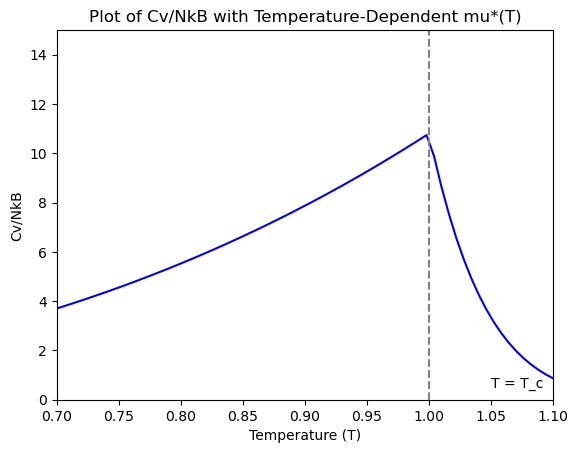
\includegraphics[width=0.7\textwidth]{output.png}
\end{center}
The specific heat exhibits a peak near the condensation temperature, reflecting the transition from a thermal distribution to a condensed state. The peak height and width depend on the number of particles and the functional form of the chemical potential.
\section{Conclusion}
In this project, we have analyzed the behavior of a Bose-Einstein condensate confined in an anisotropic harmonic potential. We have computed the density of states for both isotropic and anisotropic potentials, and discussed the implications of neglecting the ground state contribution term. We have also calculated the condensation temperature and the condensation fraction, which provide insights into the transition to a condensed state. Finally, we have derived the specific heat as a function of temperature and the number of particles, and discussed the relation between the chemical potential and the number of particles. The specific heat exhibits a peak near the condensation temperature, reflecting the transition from a thermal distribution to a condensed state. The peak height and width depend on the number of particles and the functional form of the chemical potential.\\

The results obtained in this project provide a comprehensive understanding of the behavior of a Bose-Einstein condensate in an anisotropic harmonic potential. The analysis of the density of states, condensation temperature, condensation fraction, and specific heat sheds light on the transition to a condensed state and the thermodynamic properties of the system. The insights gained from this project can be applied to further studies of Bose-Einstein condensation and related phenomena in quantum systems.\\
% \bibliographystyle{plain}  % or use other styles like apsrev4-1
% \bibliography{references}  % references.bib is the name of your .bib file

\end{document}
